\section{Time Series Analysis}

\subsection{Data Understanding}

The dataset consists of 1134 films, each represented by a time series of daily domestic 
box-office gross revenues in the United States and Canada, spanning 100 days from release day (day 0) 
to day 99. Each observation also includes descriptive metadata. The dataset contains 104 attributes in 
total: 100 numerical columns corresponding to daily gross revenues, one numerical column for the IMDb average \texttt{rating}, 
and three categorical columns identifying the film \texttt{id}, \texttt{genre}, and \texttt{rating category}.

Preliminary inspection revealed no missing values. For films with runs shorter than 100 days, 
missing entries were completed through a synthetic extension procedure, which imputes values using a noise-augmented mean 
of the observed revenues. This ensures uniform series length, although it introduces artificial values that may influence 
analyses focusing on the later days of a film's lifecycle.

Descriptive statistics provide an overview of the box-office revenue trends. 
On release day, the average revenue is approximately 9 million USD, with maximum values exceeding 150 million USD. 
Revenues decline rapidly in subsequent days, reaching mean values near 100000 USD by day 99. 
Variance remains high across the series, indicating substantial variability in revenue levels among films.
IMDb ratings show a mean of 6.6 with a standard deviation of 0.9, ranging from 2.8 to 8.7.
The \texttt{rating\_category} variable, which will serve as the target for the classification part, 
is distributed across five classes: 
\begin{itemize}
    % Low (10 titles), Medium Low (128), Medium (387), Medium High (232), and High (377). 
    \item \textbf{Low} (10 titles), representing ratings ranging from
    1.0 to 4.0;
    \item \textbf{Medium Low} (128 titles), representing ratings ranging from 4.1 to 5.5;
    \item \textbf{Medium} (387 titles), representing ratings ranging from 5.6 to 6.5;
    \item \textbf{Medium High} (232 titles), representing ratings from 6.6 to 7.0;
    \item \textbf{High} (377 titles), representing ratings from 7.1 to 10.0.
\end{itemize}
The distribution is highly imbalanced, with the Low category being significantly underrepresented compared to the other classes.


The presence of extreme values and synthetic extensions may necessitate normalization to ensure comparability 
of the time series and support more robust analyses.


% aggiungere parte di scaling eventuale o cose simili di preparation

\subsection{Motifs and Anomalies Discovery}



\subsection{Clustering}

\subsection{Classification}

The classification task aims to predict the \texttt{rating\_category} of a film based on its daily box-office revenue time series.
This category originally had five classes: Low, Medium Low, Medium, Medium High, and High.
However, due to the significant class imbalance, with the Low category containing only 10 instances,
the decision was made to merge the Low and Medium Low categories into a single class.


\subsubsection{Recurrent Neural Network}

As the last model, a Recurrent Neural Network (RNN) was
implemented, because of the suitability of RNNs for
sequential data.
Its architecture is shown in Figure~\ref{fig:rnn_model}.

\begin{figure}[H]

    \begin{minipage}{0.49\textwidth}
        The architecture was obtained through experimentation with
        different configurations and hyperparameters.
        The test and validation sets used 40\% of the dataset each,
        while the training set used the remaining 60\%.
        The split was stratified, to maintain class proportions across sets.

        The genre features are handled the same way as in previous Neural
        Networks (a Dense layer with 8 neurons and ReLU activation function,
        the right-most branch in figure~\ref{fig:rnn_model}).

        The time series data is processed through an encoder-decoder
        architecture, to extract relevant features from the sequences.
        The encoder processes the first half of the time series,
        with two Bidirectional LSTM layers (with 32 and 64 units respectively).
        The decoder processes the second half of the time series,
        with two Bidirectional LSTM layers (with 64 and 32 units respectively).
        The final shape resembles a diamond shape, with the number of units
        first increasing, then decreasing, to capture both local and global
        patterns in the data.
        Both the encoder and decoder use recurrent dropout of 0.3 in every layer
        for regularization.
    \end{minipage}
    \hfill
    \begin{minipage}{0.48\textwidth}
        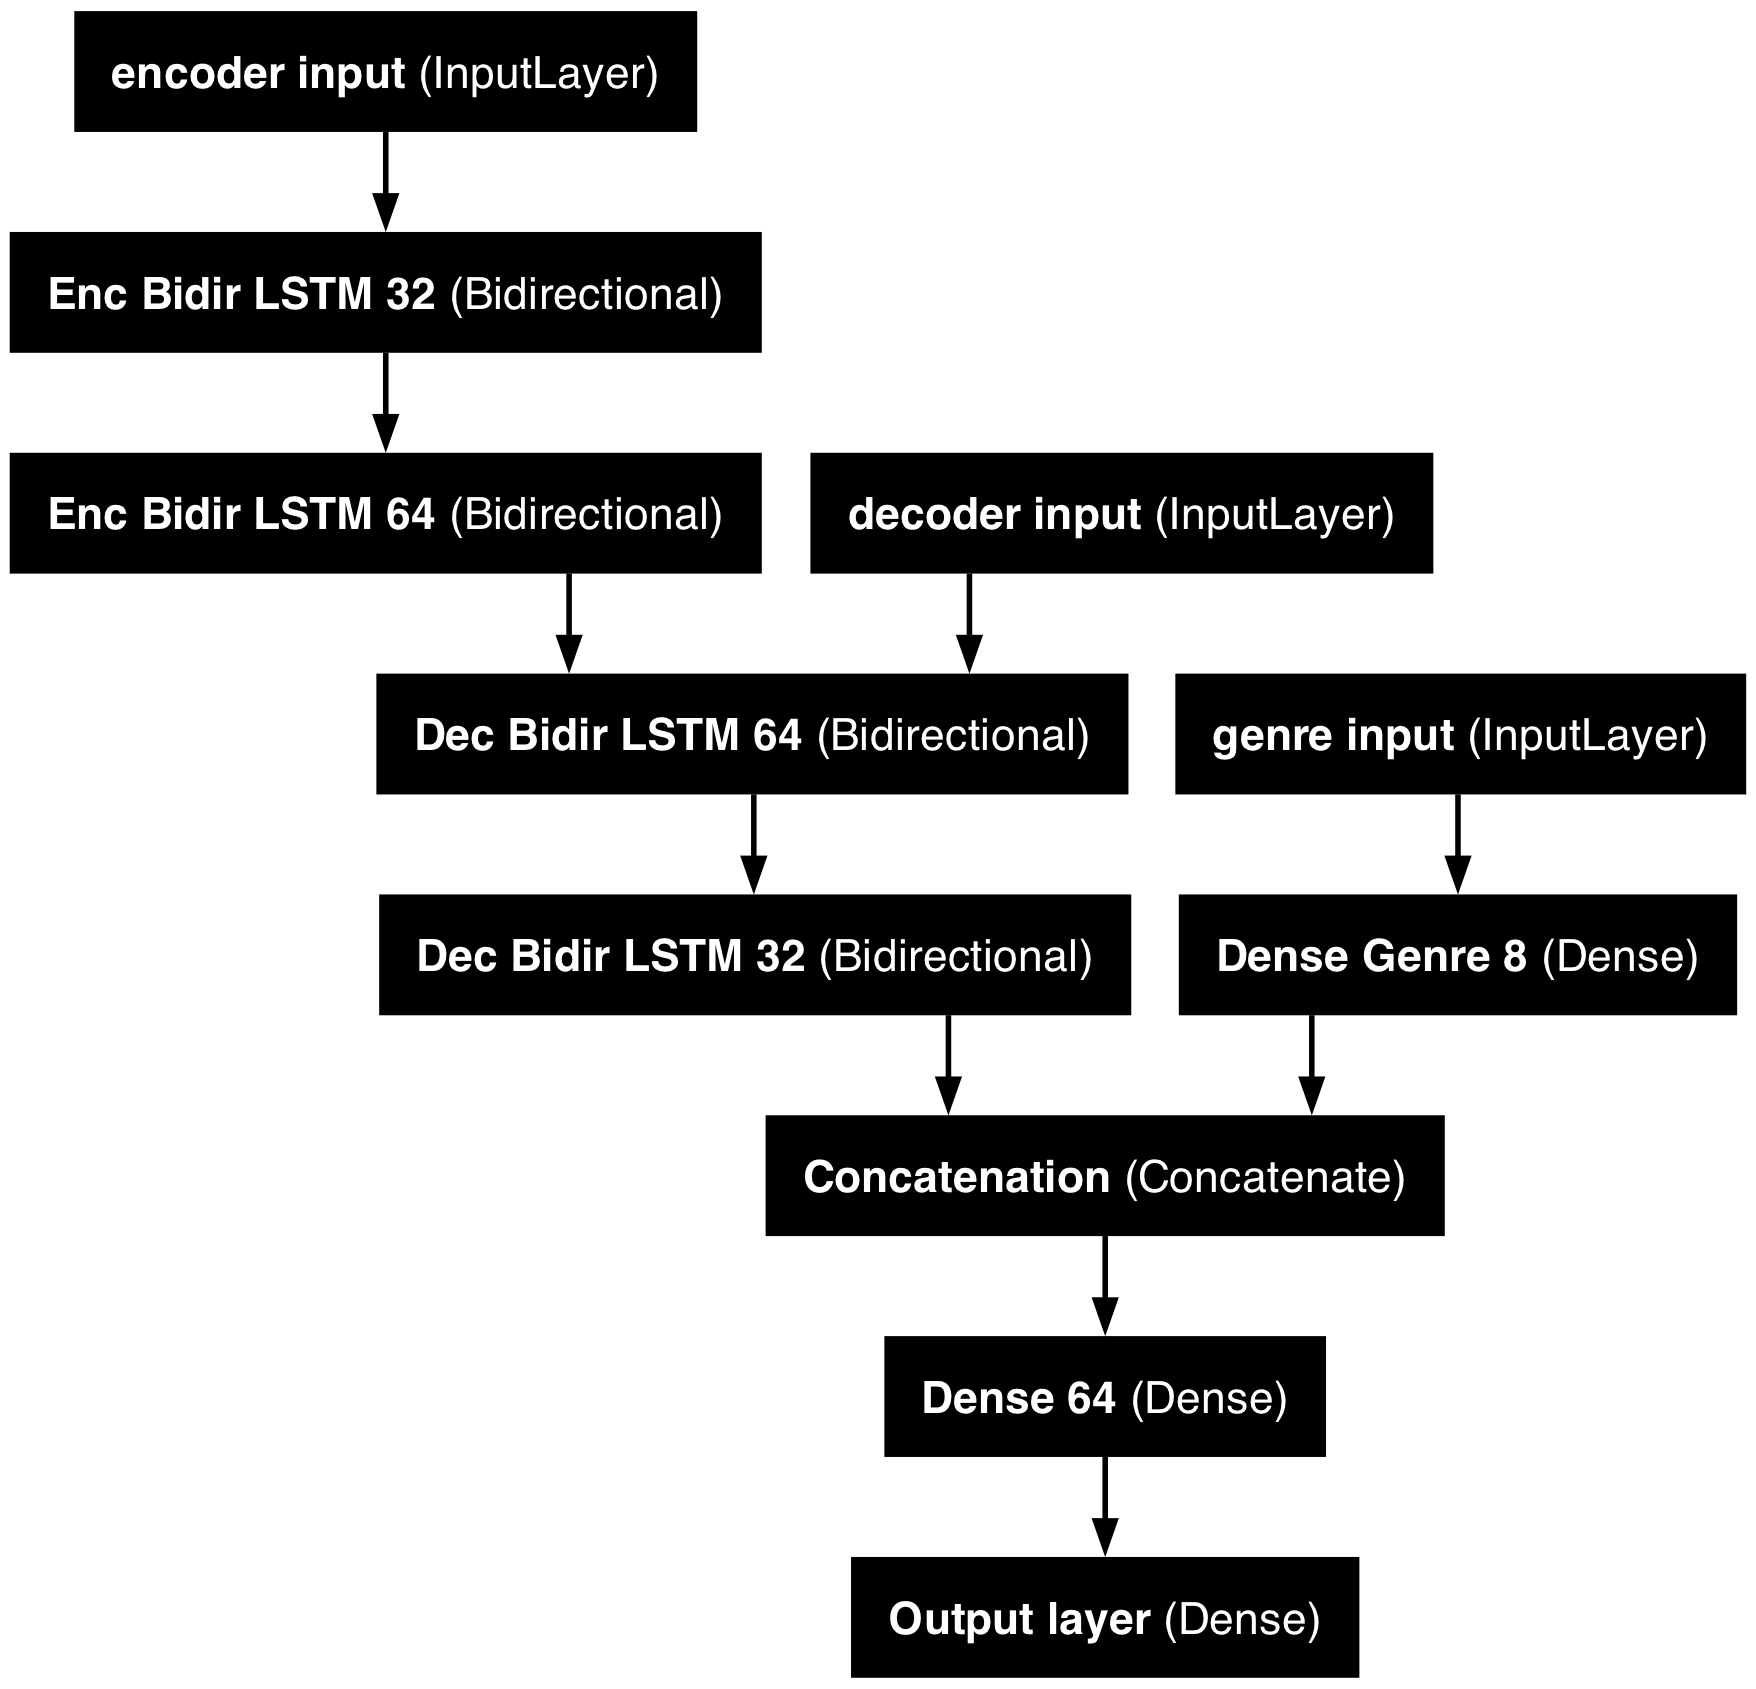
\includegraphics[width=1\textwidth]{plotsss/rnn_model.png}
        \caption{Architecture of the RNN model}
        \label{fig:rnn_model}
    \end{minipage}
\end{figure}




The outputs of the two branches are finally concatenated, and
fed to a Dense layer with 64 neurons and ReLU activation function,
followed by a Dropout layer with rate 0.3.
The final output layer has 4 neurons (one for each class)
and a Softmax activation function.
Wherever possible, Batch Normalization was applied to speed up training
and improve stability.\\

The model was trained using the Adam optimizer, categorical
cross-entropy loss function and a learning rate of 0.005.
Early stopping was employed to halt training if the validation loss
did not improve for 20 consecutive epochs.
The model was trained for a maximum of 200 epochs with a batch size
of 32, considering balanced class weights.

Figure~\ref{fig:loss_acc} shows the evolution of training and
validation loss and accuracy over epochs.
\begin{figure}[H]
    \centering
    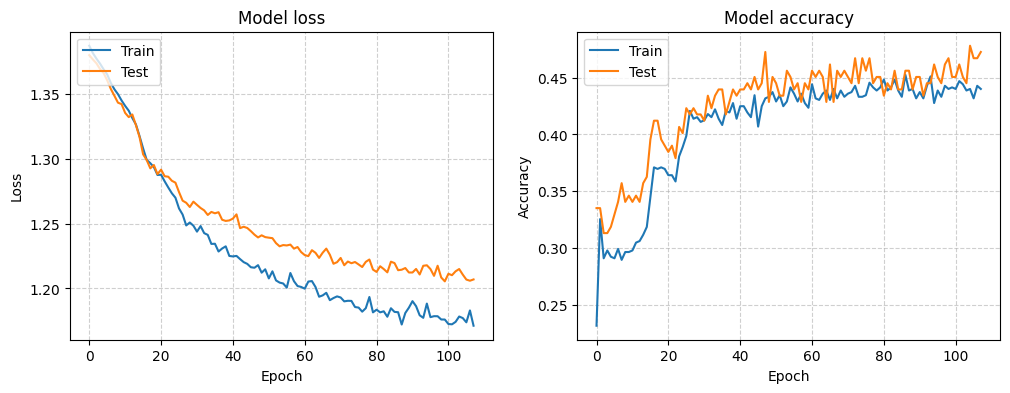
\includegraphics[width=1\textwidth]{plotsss/ts_loss_acc.png}
    \caption{Training and validation loss and accuracy over epochs}
    \label{fig:loss_acc}
\end{figure}

The loss curves show incremental improvement over epochs,
with relative stability.
Their shape do not indicate overfitting, as the validation loss
seems to find relative stability around the 50th epoch.
Accuracy curves seem to confirm that overfitting is not a central
issue.
They also show significant instability, likely due to the small
size of the dataset, which makes the small sizes of validation
and test sets more susceptible to changes in the model's behavior.


\begin{figure}[H]
    \centering
    \begin{minipage}{0.41\textwidth}
        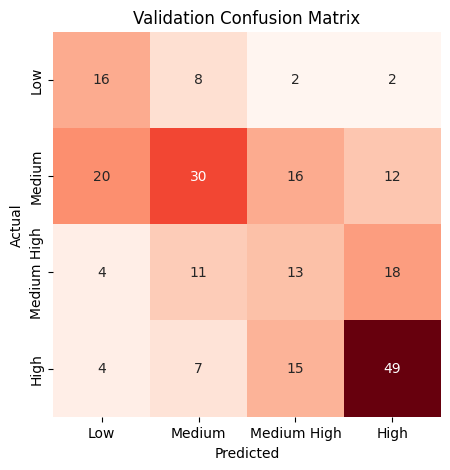
\includegraphics[width=1\textwidth]{plotsss/rnn_cm.png}
        \caption{Confusion matrix for the RNN model on the test set}
        \label{fig:cm_rnn}
    \end{minipage}
    \hfill
    \begin{minipage}{0.55\textwidth}
        Figure~\ref{fig:cm_rnn} shows the confusion matrix for the RNN
        model on the test set.

        Both \textbf{Low} and \textbf{Medium High} classes struggle
        a bit, likely because of their small size.
        Likely because of balanced class weights, both of them
        often get confused with adjacent classes.

        The \textbf{Medium} class seems to be generally hard to
        distinguish.
        It also represents the only frequent case of non-adjacent
        class misclassification, as its instances are often
        misclassified as \textbf{High}.
        This overall difficulty could be due to high overlap between
        this class and the others.
    \end{minipage}
\end{figure}

Table~\ref{tab:macro_weighted_avg} shows the macro and weighted average precision,
recall, and F1-score for the RNN model.
The final model's accuracy represents a relatively satisfactory result,
especially considering the small size of the dataset and
class imbalance.
Both macro and weighted averages can also be considered decent,
indicating that the model performs reasonably well across all classes,
without being overly biased towards the more frequent ones.

\begin{table}[H]
    \centering
    \begin{tabular}{lccc}
        \toprule
        \textbf{Metric} & \textbf{Precision} & \textbf{Recall} & \textbf{F1-score} \\
        \midrule
        \textbf{Macro avg}    & 0.45 & 0.47 & 0.45 \\
        \textbf{Weighted avg} & 0.49 & 0.48 & 0.47 \\
        \midrule
        \textbf{Accuracy}     & & & 0.48 \\
        \bottomrule
    \end{tabular}
    \caption{Macro and weighted average precision, recall, and F1-score for the RNN model}
    \label{tab:macro_weighted_avg}
\end{table}